\documentclass{article}

\usepackage{graphicx}
\usepackage{tikz}
\usepackage{tikzsymbols}
\usetikzlibrary{calc,patterns,shapes.geometric}
\pagestyle{empty}
\usepackage[margin=0pt]{geometry}
\geometry{papersize={14in,12in}}

\def\centerarc[#1](#2)(#3:#4:#5){\draw[#1] ($(#2)+({#5*cos(#3)},{#5*sin(#3)})$) arc (#3:#4:#5);}

\begin{document}
	\begin{figure}
		\centering
		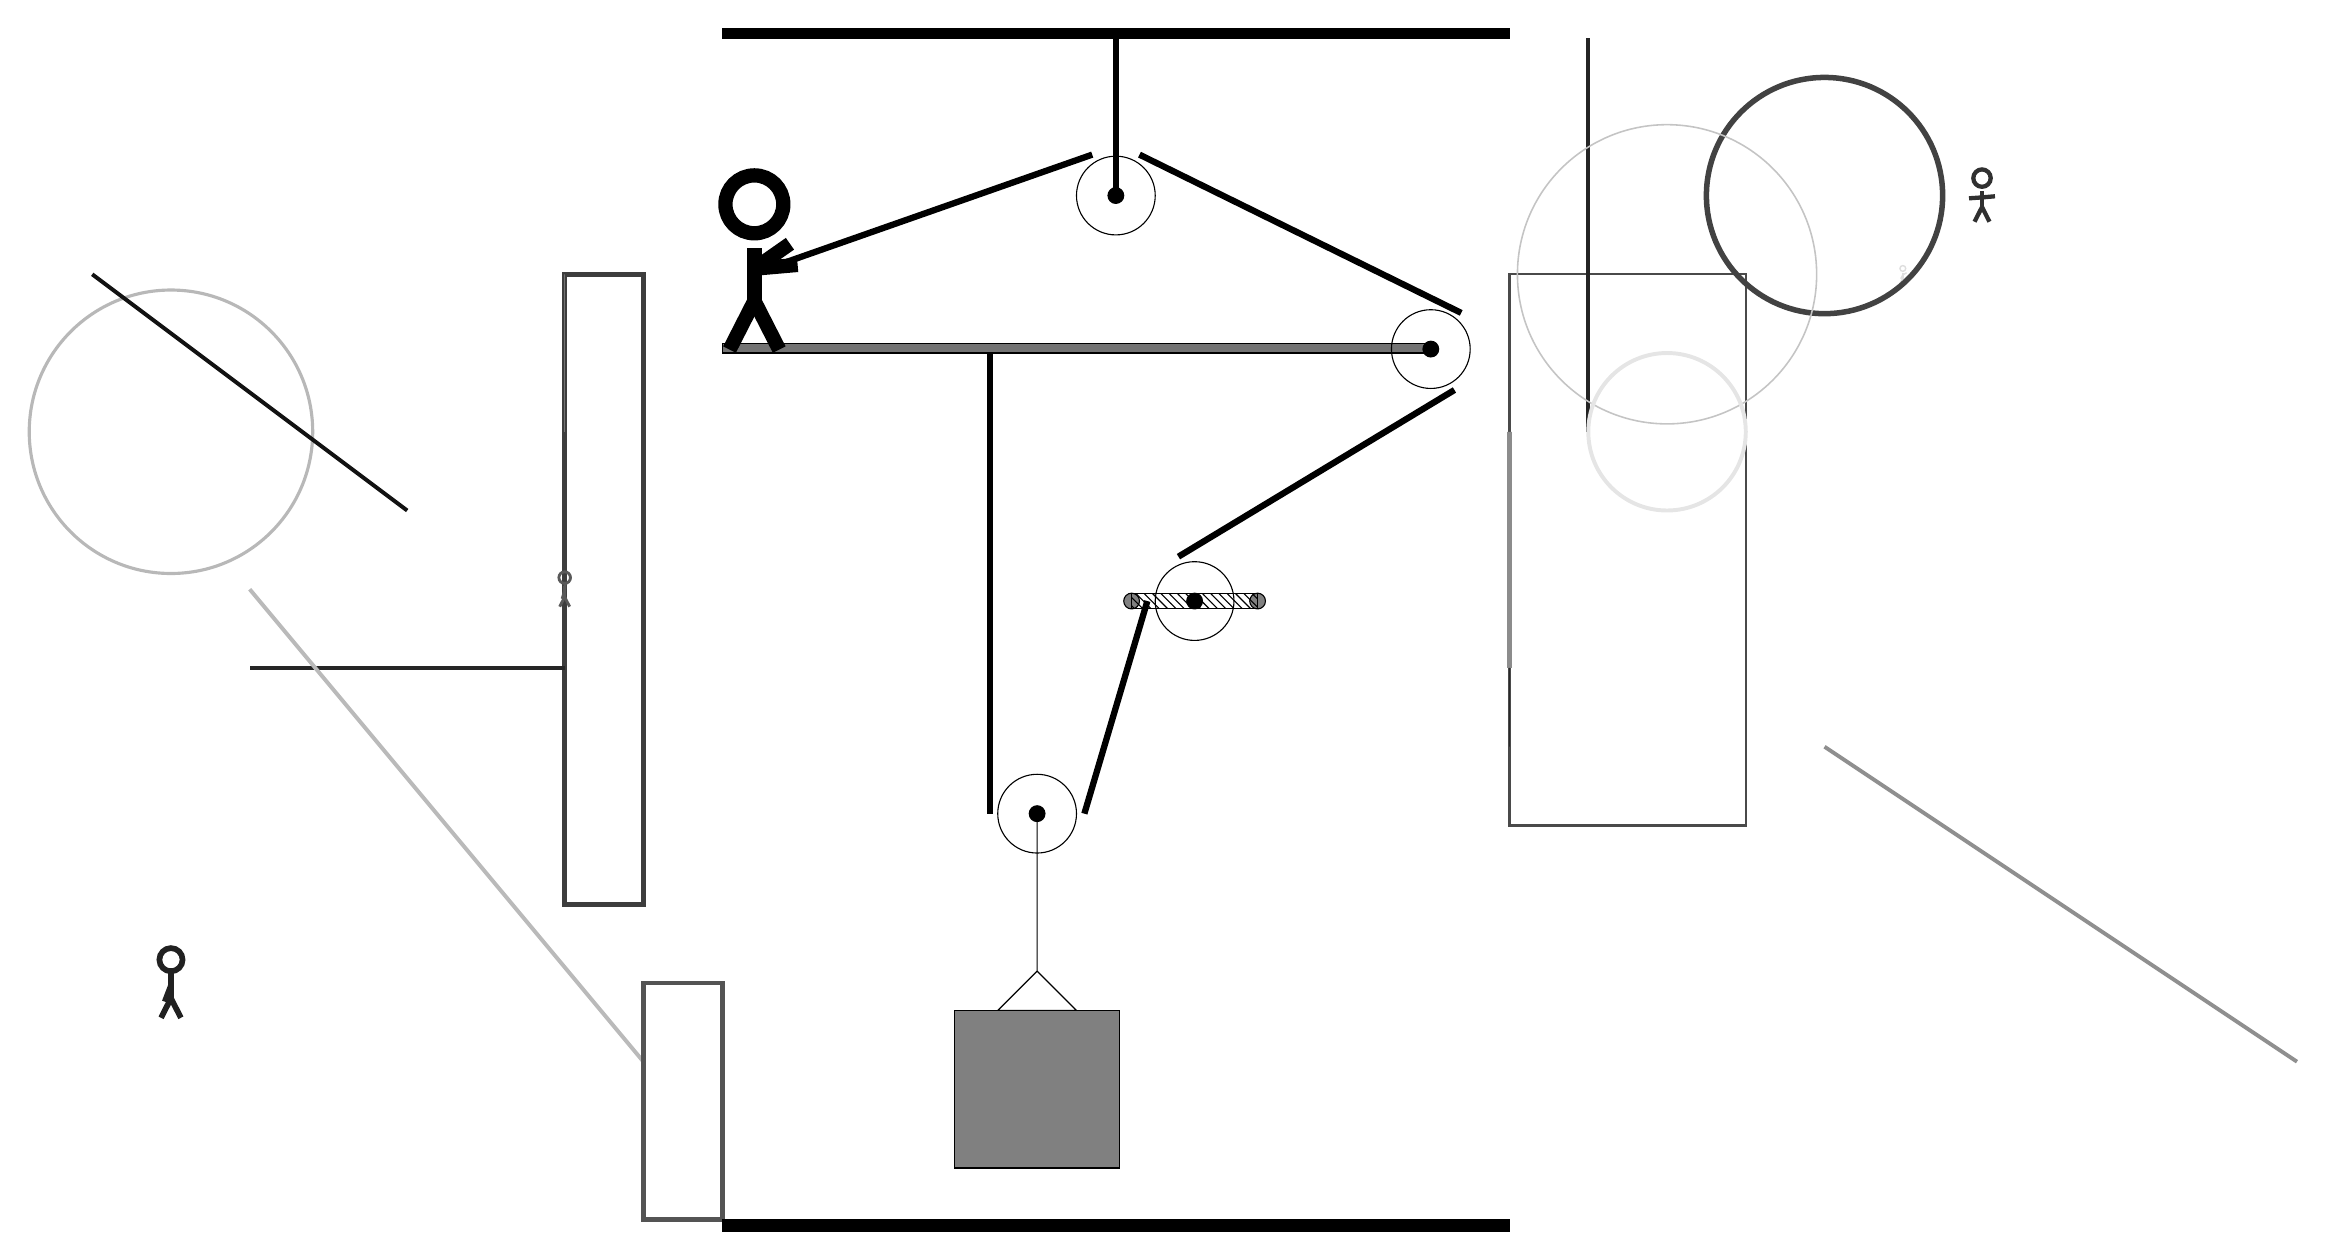
\begin{tikzpicture}
			%%%%% START %%%%%
			
			\draw[fill=black] (-2, 13) rectangle (8, 13.125);
			
			\draw[fill=black!55] (-2, 9) rectangle (7, 9.125);
			
			\draw (2, 3.15) circle (0.5);
			\draw[fill=black] (2, 3.15) circle (0.1);
			
			\draw (7, 9.05) circle (0.5);
			\draw[fill=black] (7, 9.05) circle (0.1);
			
			\draw[fill=white](4, 5.85) circle (0.5);
			\draw[fill=black] (4, 5.85) circle (0.1);
			\draw[fill=black!50] (3.2, 5.85) circle (0.1);
			\draw[fill=black!50] (4.8, 5.85) circle (0.1);
			\draw[pattern=north west lines, pattern color=black] (3.2, 5.95) rectangle (4.8, 5.75);
			
			\draw (3, 11) circle (0.5);
			\draw[fill=black] (3, 11) circle (0.1);
			\draw[line width=0.8mm] (3, 11) -- (3, 13);
			
			\draw (2, 3.15) -- (2, 1.15) -- (1.5, 0.65) -- (2.5, 0.65) -- (2, 1.15);
			\draw[fill=black!50] (0.95, 0.65) rectangle (3.05, -1.35);
			
			\node[line width=0.6mm, color=black!13] at (13, 10) {\Strichmaxerl[1][61][30]};
			
			\draw[line width=0.6mm, color=black!76] (-4, 2) rectangle (-3, 10);
			\draw[line width=0.3mm, color=black!71] (8, 10) rectangle (11, 3);
			\draw[line width=0.5mm, color=black!44](12, 4) -- (18, 0);
			\node[line width=0.4mm, color=black!65] at (-4, 6) {\Strichmaxerl[2][73][86]};
			
			\draw[line width=0.5mm, color=black!85](-4, 5) -- (-8, 5);
			\draw[line width=0.5mm, color=black!86] (9, 13) rectangle (9, 8);
			
			\draw[line width=0.6mm, color=black!45] (8, 5) rectangle (8, 8);
			\draw[line width=0.2mm, color=black!84] (8, 5) rectangle (8, 4);
			
			\node[line width=0.2mm, color=black!87] at (-9, 1) {\Strichmaxerl[4][69][90]};
			
			\draw [line width=0.4mm, color=black!28](-9, 8) circle (1.8);
			\draw[line width=0.5mm, color=black!93](-6, 7) -- (-10, 10);
			\node[line width=0.5mm, color=black!81] at (14, 11) {\Strichmaxerl[3][4][5]};
			
			\draw [line width=0.7mm, color=black!74](12, 11) circle (1.5);
			\draw[line width=0.5mm, color=black!27](-3, 0) -- (-8, 6);
			\draw [line width=0.2mm, color=black!23](10, 10) circle (1.9);
			
			\draw [line width=0.5mm, color=black!10](10, 8) circle (1.0);
			\draw[line width=0.6mm, color=black!67] (-3, 1) rectangle (-2, -2);
			\draw[line width=0.2mm, color=black!55] (-4, 8) rectangle (-4, 10);
			
			\draw[line width=0.8mm] (1.4, 9) -- (1.4, 3.15);
			\centerarc[line width=0.8mm](2, 3.15)(180:360:0.6);
			\draw[line width=0.8mm](2.6, 3.15) -- (3.4, 5.85);
			\centerarc[line width=0.8mm](4, 5.85)(110:180:0.6);
			\draw[line width=0.8mm](3.7948, 6.4138) -- (7.3, 8.5304);
			\centerarc[line width=0.8mm](7, 9.05)(-60:50:0.6);
			\draw[line width=0.8mm](7.3857, 9.5096) -- (3.3, 11.5196);
			\centerarc[line width=0.8mm](3, 11)(60:120:0.6);
			\draw[line width=0.8mm](2.7, 11.5196) -- (-1.2, 10.15);
			
			\node at (-1.5, 10.15) {\Strichmaxerl[10][-175][35]};
			
			\draw[fill=black] (-2, -2) rectangle (8, -2.15);
			
			%%%%% END %%%%%
		\end{tikzpicture}
	\end{figure}	
\end{document}